% !TeX spellcheck = en_GB
% !TEX program = xelatex+makeindex+bibtex
% !TeX TXS-program:pdflatex = txs:///xelatex %
\documentclass[final,a4paper]{report} %scrreprt of scrartcl
%!TEX program=xelatex+makeindex+bibtex
% Include all project wide packages here.
\usepackage{fullpage}
\usepackage{polyglossia}
\setmainlanguage{english}
\usepackage{csquotes}
\usepackage{graphicx}
\usepackage{epstopdf}
\usepackage{pdfpages}
\usepackage{caption}
\usepackage[list=true]{subcaption}
\usepackage{float}
\usepackage{standalone}
\usepackage{import}
\usepackage{tocloft}
\usepackage{wrapfig}
\usepackage{authblk}
\usepackage{array}
\usepackage{booktabs}
\usepackage[toc,page,title,titletoc]{appendix}
\usepackage{xunicode}
\usepackage{fontspec}
\usepackage{pgfplots}
\usepackage{SIunitx}
\usepackage{units}
\pgfplotsset{compat=newest}
\pgfplotsset{plot coordinates/math parser=false}
\newlength\figureheight 
\newlength\figurewidth
\usepackage{amsmath}
\usepackage{mathtools}
\usepackage{unicode-math}
\usepackage{rotating}
\usepackage{fancyhdr}
\usepackage{titlesec}
\usepackage{blindtext}
\usepackage{color}
\usepackage[margin=3.5cm,headheight=35pt]{geometry}
\usepackage[
    backend=bibtexu,
	texencoding=utf8,
bibencoding=utf8,
    style=ieee,
    sortlocale=en_US,
    language=auto
]{biblatex}
\usepackage{listings}
\usepackage{wrapfig}
\newcommand{\includecode}[4][c]{\lstinputlisting[caption=#2, escapechar=, style=#1,label=#4]{#3}}
\newcommand{\superscript}[1]{\ensuremath{^{\textrm{#1}}}}
\newcommand{\subscript}[1]{\ensuremath{_{\textrm{#1}}}}


\newcommand{\chapternumber}{\thechapter}
\renewcommand{\appendixname}{Appendix}
\renewcommand{\appendixtocname}{Appendices}
\renewcommand{\appendixpagename}{Appendices}

\usepackage[hidelinks]{hyperref} %<--------ALTIJD ALS LAATSTE

%!TEX program=xelatex+makeindex+bibtex
\renewcommand{\familydefault}{\sfdefault}

\setmainfont[Ligatures=TeX]{Calibri}
\setmathfont{Asana Math}
\setmonofont{Lucida Console}

%\definecolor{chapterbarcolor}{cmyk}{.52,.32,0,0}
%\definecolor{footrulecolor}{cmyk}{.52,.32,0,0}

\definecolor{chapterbarcolor}{gray}{0.75}
\definecolor{footrulecolor}{gray}{0.75}

\fancypagestyle{plain}{%
  \fancyhf{}    
  \fancyfoot[L]{\ifnum\value{chapter}>0 \chaptername\ \thechapter. \fi}
  \fancyfoot[C]{\thepage}
  \fancyfoot[R]{\small \today}
  \renewcommand{\headrulewidth}{0pt}
  \renewcommand{\footrulewidth}{2pt}
  \renewcommand{\footrule}{\hbox to\headwidth{%
  \color{footrulecolor}\leaders\hrule height \footrulewidth\hfill}}
}

\pagestyle{plain}

\newcommand{\hsp}{\hspace{20pt}}
\titleformat{\chapter}[hang]{\Huge\bfseries}{\chapternumber\hsp\textcolor{chapterbarcolor}{|}\hsp}{0pt}{\Huge\bfseries}
\titlespacing{\chapter}{0pt}{0pt}{1pt}
\renewcommand{\familydefault}{\sfdefault}
\renewcommand{\arraystretch}{1.2}
\setlength{\headheight}{0pt} 
\setlength\parindent{0pt}
\setlength{\parskip}{0.3cm plus4mm minus3mm}
\setlength\cftaftertoctitleskip{5pt}
\setlength\cftbeforetoctitleskip{20pt}

%For code listings
\definecolor{black}{rgb}{0,0,0}
\definecolor{browntags}{rgb}{0.65,0.1,0.1}
\definecolor{bluestrings}{rgb}{0,0,1}
\definecolor{graycomments}{rgb}{0.4,0.4,0.4}
\definecolor{redkeywords}{rgb}{1,0,0}
\definecolor{bluekeywords}{rgb}{0.13,0.13,0.8}
\definecolor{greencomments}{rgb}{0,0.5,0}
\definecolor{redstrings}{rgb}{0.9,0,0}
\definecolor{purpleidentifiers}{rgb}{0.01,0,0.01}


\lstdefinestyle{csharp}{
language=[Sharp]C,
showspaces=false,
showtabs=false,
breaklines=true,
showstringspaces=false,
breakatwhitespace=true,
escapeinside={(*@}{@*)},
columns=fullflexible,
commentstyle=\color{greencomments},
keywordstyle=\color{bluekeywords}\bfseries,
stringstyle=\color{redstrings},
identifierstyle=\color{purpleidentifiers},
basicstyle=\ttfamily\small}

\lstdefinestyle{c}{
language=C,
showspaces=false,
showtabs=false,
breaklines=true,
showstringspaces=false,
breakatwhitespace=true,
escapeinside={(*@}{@*)},
columns=fullflexible,
commentstyle=\color{greencomments},
keywordstyle=\color{bluekeywords}\bfseries,
stringstyle=\color{redstrings},
identifierstyle=\color{purpleidentifiers},
}

\lstdefinestyle{matlab}{
language=Matlab,
showspaces=false,
showtabs=false,
breaklines=true,
showstringspaces=false,
breakatwhitespace=true,
escapeinside={(*@}{@*)},
columns=fullflexible,
commentstyle=\color{greencomments},
keywordstyle=\color{bluekeywords}\bfseries,
stringstyle=\color{redstrings},
identifierstyle=\color{purpleidentifiers}
}

\lstdefinestyle{vhdl}{
language=VHDL,
showspaces=false,
showtabs=false,
breaklines=true,
showstringspaces=false,
breakatwhitespace=true,
escapeinside={(*@}{@*)},
columns=fullflexible,
commentstyle=\color{greencomments},
keywordstyle=\color{bluekeywords}\bfseries,
stringstyle=\color{redstrings},
identifierstyle=\color{purpleidentifiers}
}

\lstdefinestyle{xaml}{
language=XML,
showspaces=false,
showtabs=false,
breaklines=true,
showstringspaces=false,
breakatwhitespace=true,
escapeinside={(*@}{@*)},
columns=fullflexible,
commentstyle=\color{greencomments},
keywordstyle=\color{redkeywords},
stringstyle=\color{bluestrings},
tagstyle=\color{browntags},
morestring=[b]",
  morecomment=[s]{<?}{?>},
  morekeywords={xmlns,version,typex:AsyncRecords,x:Arguments,x:Boolean,x:Byte,x:Char,x:Class,x:ClassAttributes,x:ClassModifier,x:Code,x:ConnectionId,x:Decimal,x:Double,x:FactoryMethod,x:FieldModifier,x:Int16,x:Int32,x:Int64,x:Key,x:Members,x:Name,x:Object,x:Property,x:Shared,x:Single,x:String,x:Subclass,x:SynchronousMode,x:TimeSpan,x:TypeArguments,x:Uid,x:Uri,x:XData,Grid.Column,Grid.ColumnSpan,Click,ClipToBounds,Content,DropDownOpened,FontSize,Foreground,Header,Height,HorizontalAlignment,HorizontalContentAlignment,IsCancel,IsDefault,IsEnabled,IsSelected,Margin,MinHeight,MinWidth,Padding,SnapsToDevicePixels,Target,TextWrapping,Title,VerticalAlignment,VerticalContentAlignment,Width,WindowStartupLocation,Binding,Mode,OneWay,xmlns:x}
}

%defaults
\lstset{
basicstyle=\ttfamily\scriptsize ,
extendedchars=false,
numbers=left,
numberstyle=\ttfamily\tiny,
stepnumber=1,
tabsize=4,
numbersep=5pt
}
\addbibresource{../../library/bibliography.bib}
\author{Fairphone Repair Group}
\title{Fairphone Repairability}
\date{\today}
\begin{document}
	\chapter{SCRW-It}
	\label{ch:scrw-it}
	The second product the team decided to develop is not the main product. In fact, it is actually more of a gadget. The product is the size of a credit card, and serves as a business card, Fairphone membership badge, diagnosing and repairing tool. 
	
	The first step in designing the card, was making a list of requirements:
	\begin{enumerate}
		\item Must fit in a walled
		\item Must have \#000 Philips screwdriver
		\item Must be identifiable as a Fairphone product and serve as a membership badge
		\item Must be able to encase diagnosing hardware
	\end{enumerate}
	
	\section{The first design}
	\label{sec:scrw-it-first-design}
	
	The first design phase served to make sure requirements 1 to 3 were met. It wasn't certain whether it was possible to meet requirements 1 and 4, since more research was required before anything could be said about it (Section \ref{sec:scrw-it-hardware}). 
	
	Figure \ref{fig:CardExteriorDesign} shows the exterior of the card. It has a logo similar to Fairphone's, but instead of the star it pictures an open end wrench symbolizing the repairing function it provides. The figure also shows a narrow detachable section with two screwdrivers (one the required Philips and the other a slot, torx or any type of screwdriver Fairphone chooses to provide) attached to it. The screwdrivers give the product its name: the SCRW-It. This is meant to be funny to lighten the user with the broken phone's mood while he repairs his phone\footnote{The screwdrivers in the prototype are a lot larger than they are supposed to be because the prototype is 3D printed whereas the real product would have a different production method and have steel screwdrivers of the correct size.}. 
	
	The previously mentioned component is made of aluminium for light weight and sufficient torquing strength for unscrewing the tiny screws. It is detachable from the rest of the card for ergonomic reasons and to avoid cracking in the plastic part of the card.
	
	\begin{figure}[H]
		\centering
		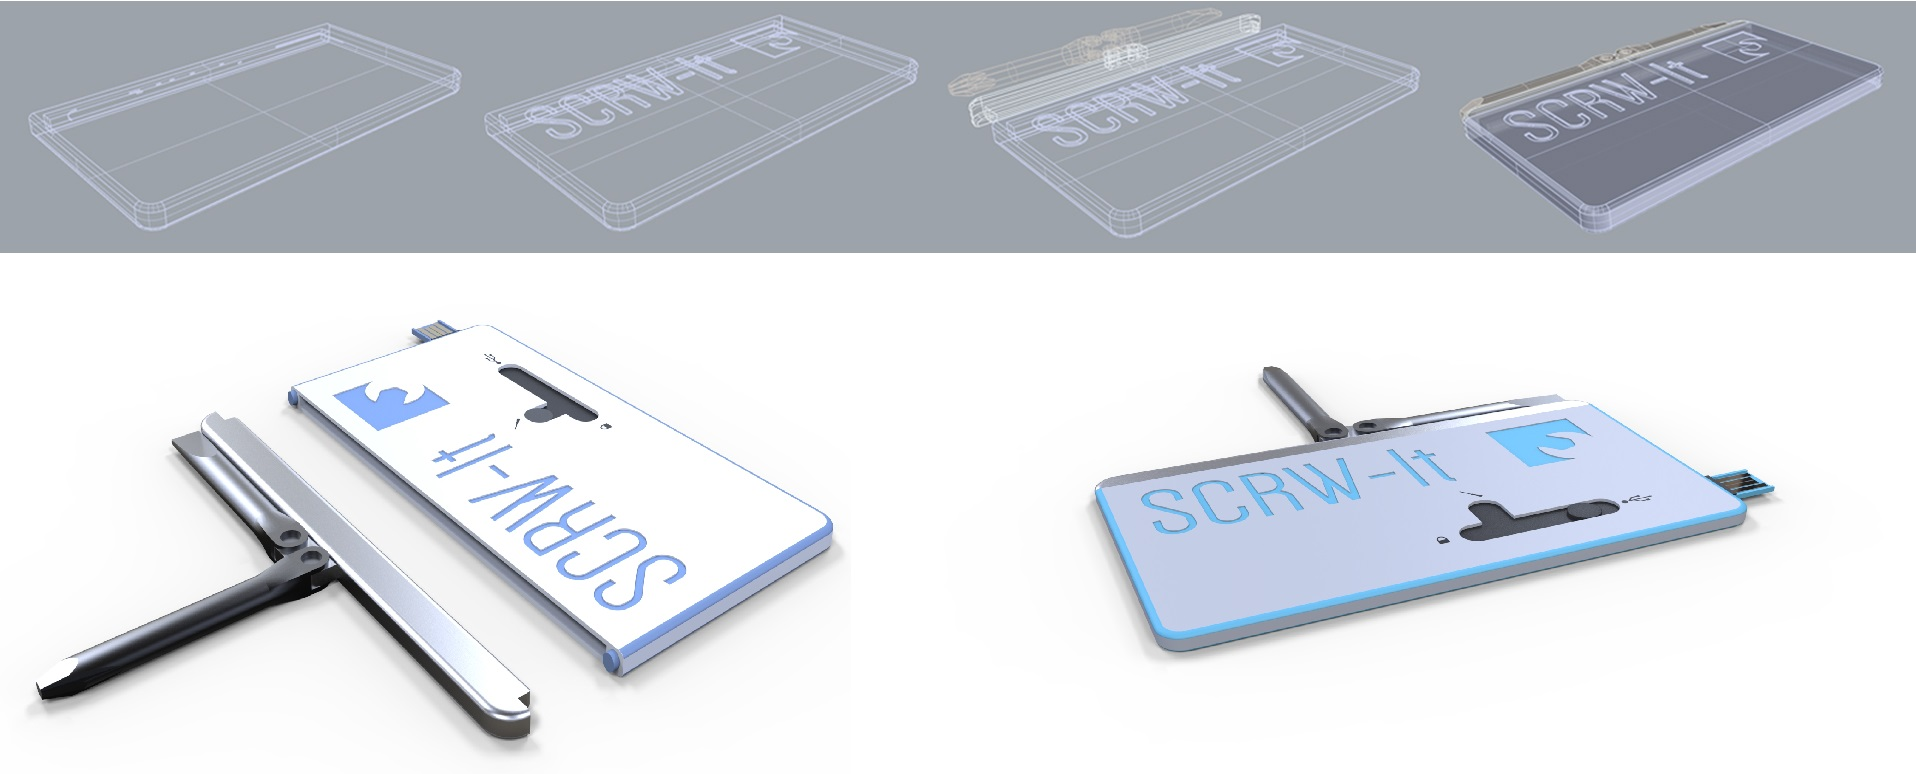
\includegraphics[width=0.8\textwidth]{resources/CardDesign1}
		\caption{Card exterior design}
		\label{fig:CardExteriorDesign}
	\end{figure}
	
	Figure \ref{fig:CardExteriorDesign} also shows a slot on the lower right side. This part is better explained in figure \ref{fig:CardInteriorDesign} where the inside is visible. The black component serves as a USB drive and a force pin to detach the aluminium part from the rest of the card. It can in fact be slid in three directions: left to access the USB drive which will stick out of the side of the card, up to detach the screwdrivers and right to lock the card when it is not in use. 
	
	\begin{figure}[H]
		\centering
		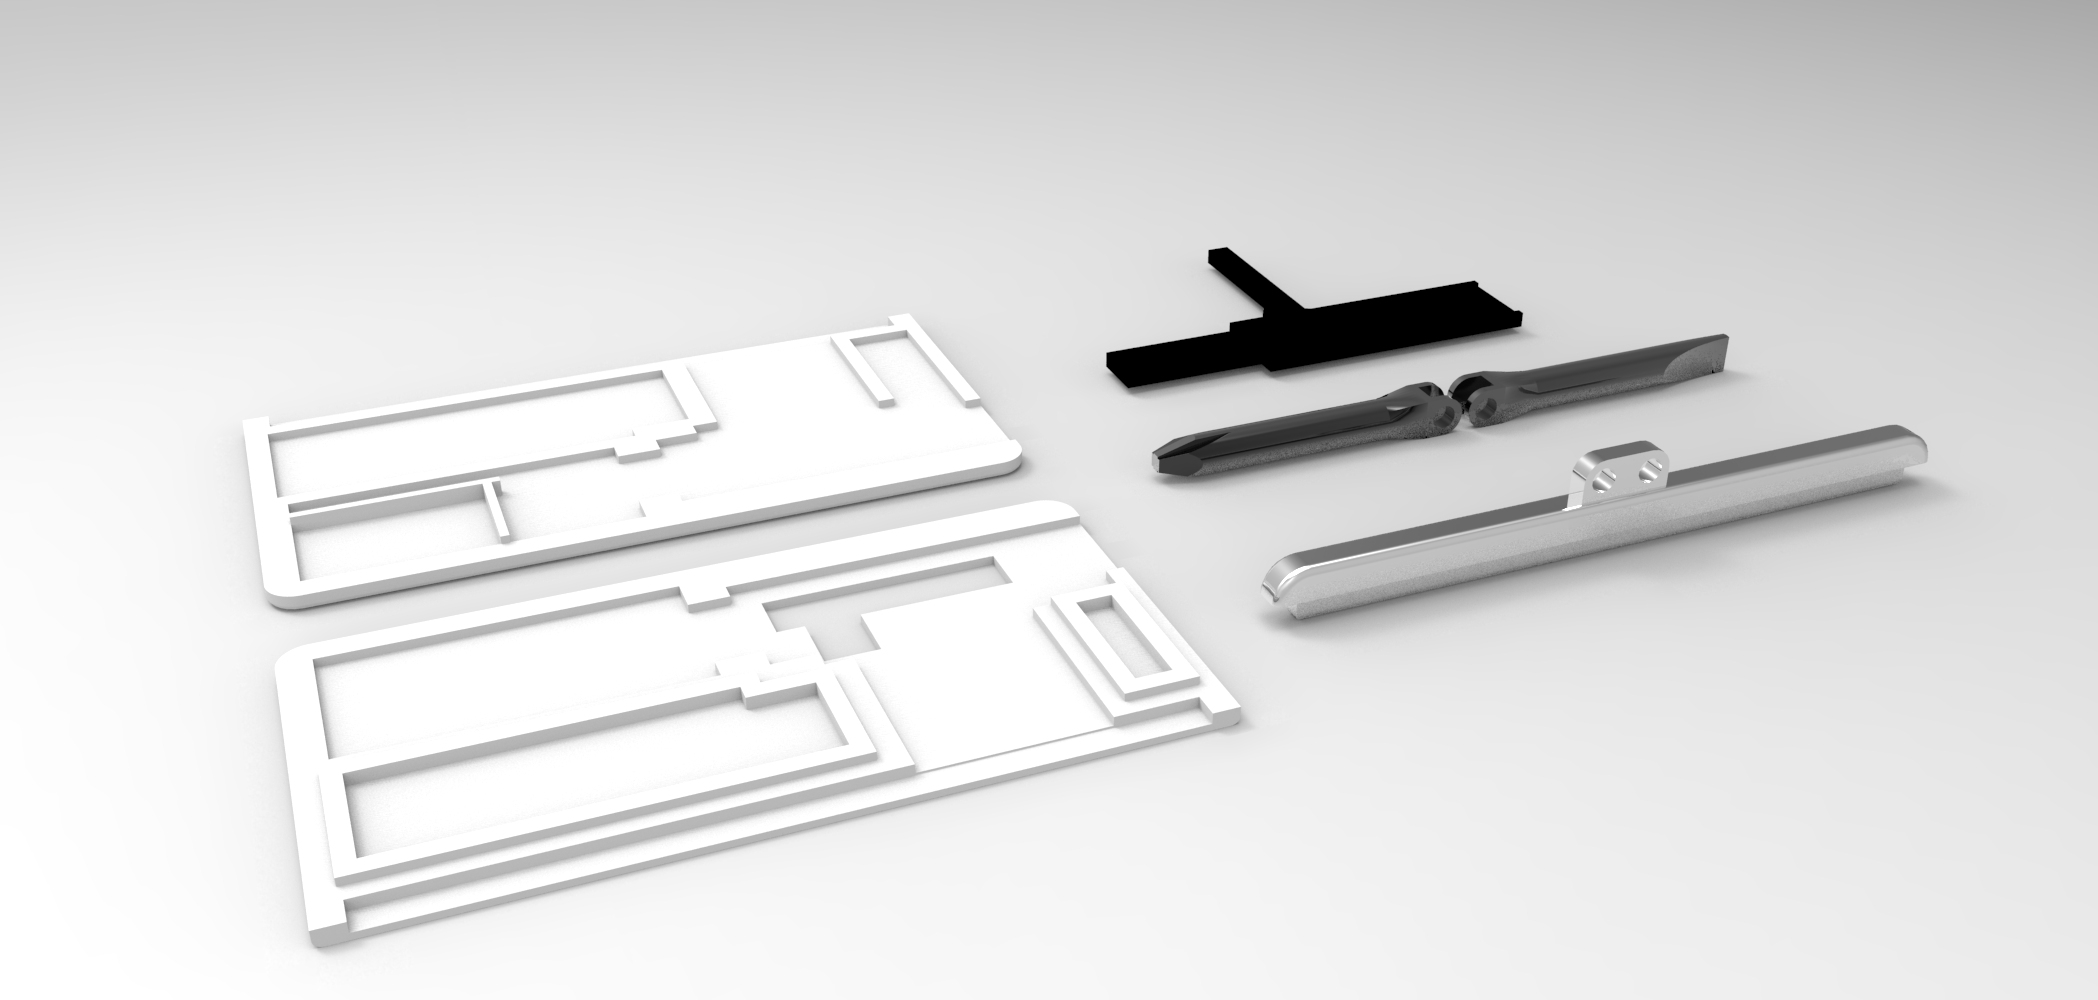
\includegraphics[width=0.8\textwidth]{resources/CardDesign2}
		\caption{Card interior design}
		\label{fig:CardInteriorDesign}
	\end{figure}
	
	This first design was made in case requirements 1 and 4 could not be met in the same product, which would have resulted in the removal of the fourth requirement. However, it was possible to meet all requirements and thus bring forward a new design (Section \ref{sec:scrw-it-hardware}).
	
	\subimport{user-testing/}{user-testing.tex}
	\subimport{feedback/}{feedback.tex}
	\subimport{improvements/}{improvements.tex}
	\subimport{hardware/}{hardware.tex}
\end{document}

